\chapter{Flash Analysis}
\label{chp:Flash_Analysis}
The goal of the flash analyser, as explained earlier, is to capture the flash and extract useful features. 
Before we are able to analyse flashes we have to find the ideal flash-generator settings. For this reason the first section of this chapter focuses on finding the ideal flash settings. The second section will focus on how and what kind of features to extract from the flash. The final section will show the variance still left in the signal.



\section{Flash generator settings}
\label{sec:Flash_generator}
The flash generator has several parameters which can be changed: T (period), t-on (on time of the LED) and I (brightness of the LED).

In order to find the ideal flash settings we use the test set-up shown in figure \ref{fig:Flashcapturing}. D in the figure represents the distance between the device and the reflecting surface. 

\begin{figure}
	\centering     %%% not \center
	\label{fig:Flashcapturing}
	\subfigure[Test setup in illuminated environment]{\label{fig:a}\includegraphics[width=60mm]{pics/Flashcapture_light.png}}
	\subfigure[Test setup in dark environment]{\label{fig:b}\includegraphics[width=60mm]{pics/Flashcapture_dark.png}}
	\caption{Test setup used to capture flashes in the darkroom.}
\end{figure}

% figure of flashes with different distances (0.8m, 1m, 1.2m and 1.4m)
% figure of flashes with different T-on @1m
% figure of consecutive flashes with different filters


\section{Feature extraction}

\section{Overview}



show several captured flashes. and explain what we see.
explain features extractable from the flash
 - maximum
 - minimum
 - surface under graph
 - 

show real turn on delay time (or in our case, the time we are able to sense the light), rise-time, and turn-off-delay.
Define turn on time.

\begin{figure}[]
	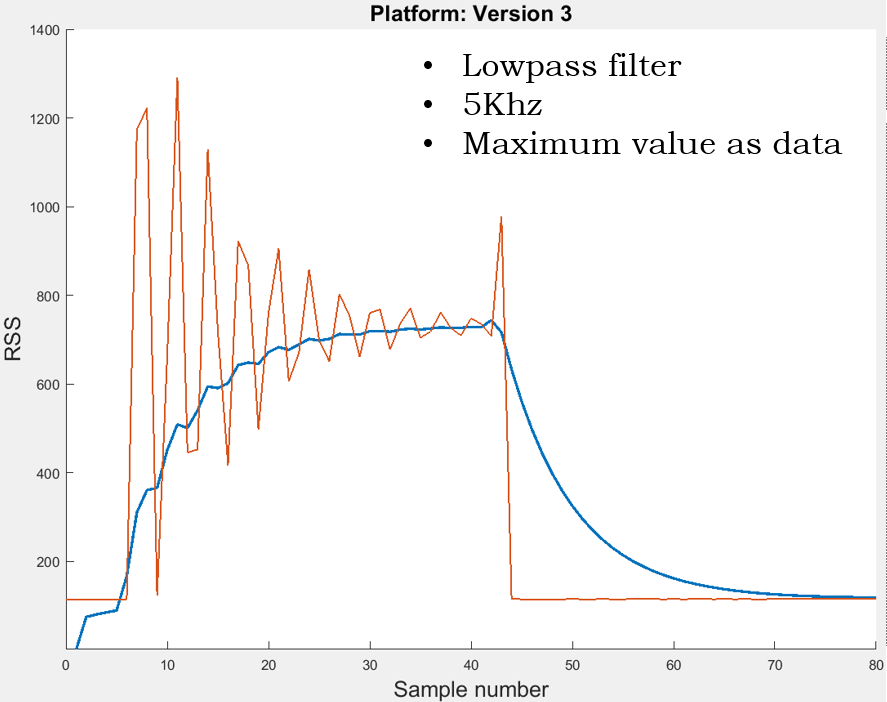
\includegraphics[width=\textwidth]{pics/66KhzFilter_placeholder.png}
	\caption{The data captured by the system before and after filtering. @=PLACEHOLDER FIGURE!@.}
	\label{fig:66KhzFilter}
\end{figure}

\subsection{Data generation}
\label{sec:Data_generation}
Show several filtered captured signals in one figure\\
point out the part where light becomes constant\\
pick that t-on time as minimum\\
Mention that a sample of darkness can be taken @ 80 samples.\\
That the number (80) can be reduced by picking a FIR filter instead (less ripple)\\

\subsection{Results and conclusion}
\label{sec:conclusion}
Show the result of several "filtered flashes\\
Explain sources of the "noise", also show FFT and histogram of the noise\\
Explain that the noise could be reduced, but that this would cost a lot more processor time. (which is not recommended to run at 125Hz).\\
Note the noise is approximately Gaussian.

\begin{figure}[!h]
	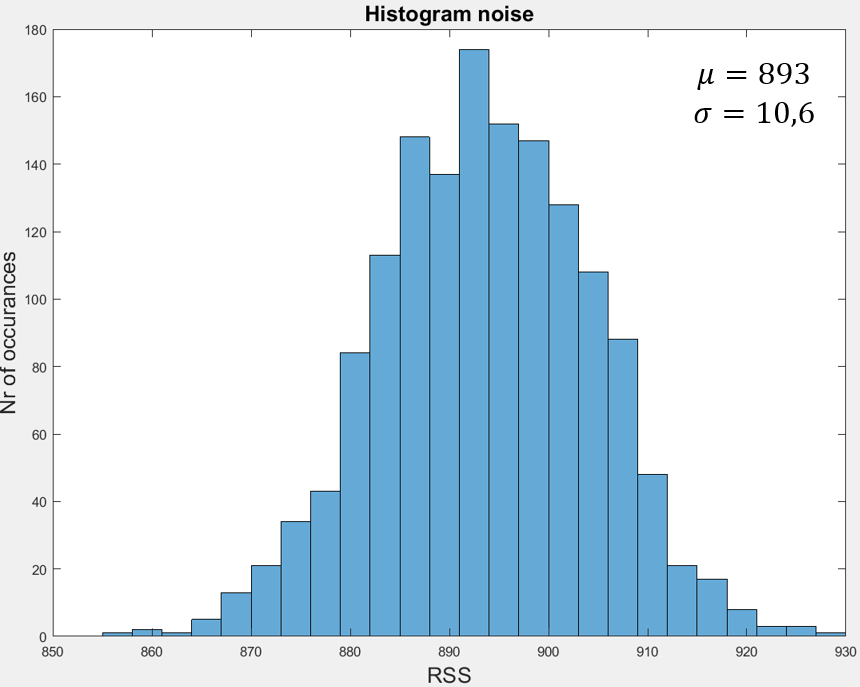
\includegraphics[width=\textwidth]{pics/histogram_noise_placeholder.png}
	\caption{Histogram of the noise of the data sampled by the system. The distribution roughly follows a normal curve. @=PLACEHOLDER FIGURE!@.}
	\label{fig:histogram_noise}
\end{figure}
